\documentclass[parskip]{scrartcl}
\usepackage{preamble}

% Title Page
% Definitionen für die Titelseite
% Change the content of the second bracket pair to what you need
\newcommand{\workauthor}{Thaddeus Kühn, Fiona Tanner, Frederik Racky, Dana Levi}
\newcommand{\worktitle}{Temperature sensitivity of dengue in Thailand}
\newcommand{\workyear}{2023}
\newcommand{\supervisor}{Stella Dafka}

\begin{document}

\begin{titlepage}
    % HIER NICHTS ÄNDERN SONDER BEI DEN DEFINITIONEN OBEN DRÜBER    
    {\usekomafont{title}
    {\vspace*{1cm}\Huge \worktitle{}}}
    
    \vspace{\stretch{2}}
    
    {\Large \workauthor{}}

    
    \vspace{\stretch{6}}
    
    	Bioinformatics Project group 4 team 4 climate sensitive infectious diseases Summer Term \workyear{}
    
    Supervisor: \textbf{\supervisor{}}
    
    \vspace{\stretch{4}}
   
    
    \vspace{\stretch{4}}

    
\end{titlepage}




\begin{abstract}

    The full abstract goes here
    

\end{abstract}



\tableofcontents

%    Abkürzungsverzeichnis
{\setlength{\parskip}{0.2cm}
\section*{Abbreviations}
    \begin{acronym}[LC-MS/MS23]
        % A B C D E F G H I J K L M N O P Q R S T U V W X Y Z        
        % Abkürzungen
        \acro{DHF}{Dengue Hemmorhagic Fever}
        
        % Formelzeichen
        
        
        % als benutzt markierte Acronyme    
        
        
    \end{acronym}
}
\newpage
\section{Introduction}\label{sec:introduction}

The Dengue virus is a vector borne virus, consisting of four serotypes (DENV 1-4).  It is transmitted to humans by mosquitoes, more specifically by \emph{Aedes aegypti} and \emph{Aedes albopictus} \citep{Phanitchat.2019}. The resulting infection goes asymptomatic in many cases, but can also cause Dengue Hemmorhagic Fever (DHF), characterized by symptoms like fever, headache, joint and muscle pain as well as (internal) bleeding and bruising \citep{Gubler.1998}.
Dengue is an emerging public health issue, with half of the worlds population at risk of infection. 390 million cases per year are estimated worldwide, with most of them not showing symptoms and thus not being reported. Affected areas range from sub-tropical to tropical regions, with south-east Asia, including Thailand, being one of the most seriously affected regions. Newly affected areas also include Europe \citep{WHO.2023}.
The disease control of dengue is challenging due to the absence of an effective treatment or vaccine, which leaves only the treatment of symptoms with painkillers like paracetamol \citep{WHO.2023}. Responsible institutions in affected areas currently focus on prevention, vector control, case control and prediction of possible future outbreaks \citep{Phanitchat.2019}. 

An important factor in predicting the epidemiological dynamics of Dengue is the climate: climate fluctuations due to recurring weather phenomenons and climate change are shown to influence \emph{Aedes} biology and infections \citep{Descloux2012, Phanitchat.2019}.
In several studies, maximal temperature has an effect on dengue transmission \citep{Descloux2012}, being associated with higher incidence \citep{Phanitchat.2019} between 27 °C and 29,5 °C. The temperature with the highest epidemic potential was shown to be 29,3 °C with a low temperature range throughout the day \citep{Liu2014}. Extreme global climate events like el Niño have been shown to affect disease outbreaks like Dengue as well \citep{Anyamba2019}.

In Thailand, a significant climate factor is the monsoon, which can be separated into two seasons: The south-west monsoon between may and october is characterized by higher temperature and high precipitation. The north-east monsoon between november and february is characterized by lower temperature and low precipitation \citep{Kripalani1995}. It has been shown that in northern districts of Thailand, there has been a detectable rise in temperature since the mid 20th century \citep{Masud2016}.

In this analysis, we are going to investigate the correlation between temperature and Dengue in Thailand from 2006 to 2020 to assess the significance of climate change, recurring climate fluctuations and extremes and geographical factors on Dengue infections.
It is concentrated on three main points: Time periods with DHF incidence will be compared to time points of extreme weather events. It will be examined if provinces with higher temperature also show higher incidences. The observation of trends in temperature and dengue cases over the course of the given time period will be analysed and compared. 
Based on the findings, two models will be generated to forecast the development of dengue fever cases: Autoregressive moving average (ARIMA) will be used to model the near future. Then, Generalized Additive Model (GAM) will be generated to predict the spatial distribution of incidences over Thailand in the future. 


\section{Material and Methods}

\subsection{Material}

	\paragraph{ERA5 data (climate)}
	The ERA5 database is a global climate database by the European Centre for Medium-Range Weather Forecasts (ECMWF), covering the earth in a 31 km horizontal grid up to 80 km in the atmosphere in the time period from 1950 to present. It was generated from measurements of various climate variables combined with a reanalysis of existing data and past reanalysis data to accurately model and complete the dataset in the given resolution \citep{Hersbach2020}. For this project, monthly temperature data 2m above ground for every province in Thailand in the timeframe of 2006 - 2020 was extracted.
	\paragraph{Dengue data}
	The Dengue case numbers are retrieved from annual infectious disease reports published by the Thailand ministry of health. Monthly case numbers of DHF for every province in the timeframe of 2006 - 2020 are used in this project. 
	
	The datasets are used with a resolution at province level. As of 2011, Thailand has a total of 77 provinces, but had 76 provinces before 2011, as Bueng Kan was split from Nong Khai in 2011. For better compatibility of the data before and after 2011, the two new provinces are merged into a province equivalent to Nong Khai before 2011. 
	
	\paragraph{Climate forecast}
	For GAM modeling, temperature  data from the CORDEX climate model is used. It includes the temperature 2m above ground for June to August (south west monsoon) of the years 2021 -2040 at a 22 km grid \citep{Copernicus2019}. 
	\paragraph{Population data}
	We used ... population data of every Thailand province from 2006 - 2020 (Quelle?).
	
	\paragraph{Spatial data}
	To associate our data with the different provinces and visualize it, we use spatial data of Thailand’s provinces. The two main data types in spatial data are vector-data and raster-data. Vector-data consists of a list of points with their exact location, which can then form lines or polygons. Raster-data assigns a value to every square of a raster. In this case, maps consisting of polygons for each province are used \citep{sds}. With the sf package, objects associating our data for each province with its coordinates and polygons are created, describing its shape. The function geom\_sf of ggplot2 are used for mapping. 
	
	\subsection{Methods}
	
	\paragraph{Descriptive analysis}
	Linear regression is a method to describe a linear relationship between variables, using the minimum sum of squares between regression line and data points to identify possible trends \citep{Schneider2010}. 


	\paragraph{ARIMA}
	
	To predict the development of the dengue cases with an ARIMA model, a time series with the total dengue cases of Thailand was created. 
	A requirement for fitting an ARIMA model is a stationary time-series. This is obtained when the mean value doesn’t change over time, the variance doesn’t increase and the seasonality effect is minimal. Two tests were used to test for stationarity of the data. The Augmented Dickey-Fuller (ADF) test examines whether the time series has a unit root, indicating non-stationarity. The null hypothesis assumes the presence of a unit root, implying non-stationarity, while the alternative hypothesis suggests stationarity. Therefore a p-value below the significance level supports the conclusion that the time series is stationary. On the other hand, the Kwiatkowski-Phillips-Schmidt-Shin (KPSS) test is also a unit root test but focuses on the presence of a deterministic trend in the series. The null hypothesis assumes stationarity, and a high p-value indicates that the time series is indeed stationary. In contrast to AGF-test, for the KPSS-test the null hypothesis assumes stationarity, and a high p-value indicates that the time series is indeed stationary. If the time series is initially found to be non-stationary, the differences between consecutive observations can be calculated, and the stationarity tests can be applied again. 
	ARIMA models combine an autoregressive model AR(p) and a moving average model MA(q). 
	The autoregressive model computes the current value from previous values and the error term:
	$$yt=c+\phi 1yt−1+\phi 2yt−2+⋯+\phi pyt−p+\epsilon t$$
	
	$\epsilon t$ = white noise
	$1,…,\phi p$ = parameters
	$yt-1,…, yt-p$ = lagged values 
	For the moving average the current value consists of the mean value of the time series and weighted current and past error terms: 
	yt=c+εt+θ1εt−1+θ2εt−2+⋯+θqεt−q
	θ1,…, θq = parameters
	I(t) is the number of times differencing was performed to make the time series stationary.
	To find the best values for p and q, the Autocorrelation function (ACF) and partial Autocorrelation function (pACF) can be evaluated. The ACF plot shows the correlations of a time-series with lags of itself, while the pACF additionally removes the effects of lags. 
	A second evaluation tool is the auto.arima function. It automatically fits the best ARIMA model by minimizing the Akaike’s Information Criterion (AIC). The aout.arima function can also consider seasonal models.  
	A good forecasting method will yield residuals with the following properties:
	1.	The residuals are uncorrelated. If there are correlations between residuals, then there is information left in the residuals which should be used in computing forecasts.
	2.	The residuals have zero mean. If the residuals have a mean other than zero, then the forecasts are biased.
	3.	The residuals have constant variance.
	4.	The residuals are normally distributed.
	5.	
	
	A time series can be decomposed in the components trend, seasonality and random. For additive decomposition the original time series is the sum of the different components.
	
	\paragraph{GAM}
	GAM provides insight into the shape and direction of the relationship between temperature and dengue cases. Additionally, it was used to forecast the future dengue case development based on the temperature development prediction. 
	A GAM is a flexible extension of Generalized Linear Models (GLMs) that allows for the modelling of non-linear relationships between the response variable and predictor variables. A linear model can be described as follows:
	$y=\beta _0+\beta _1 x_1+\beta _2 x_2 +…+\beta _p x_p+\epsilon$
	GAMs are now a nonparametric form of regression where the linear predictors $(\beta_i x_i)$ of the regression are replaced by smooth functions of the explanatory variables, $f(x_i)$. The model can be defined as:
	$y_i=f(x_i )+\in_i$
	where $y_i$ is the response variable, $x_i$ is the predictor variable, and f is the smooth function \citep{Wood2006}.
	It is called an additive model, because all the $f(x_i)$ functions and therefore their predictor variables contribute individually to the response variable and are added up. The advantage is that the different smooth functions can capture complex relationships by flexibly fitting curves to the data.
	There are two different ways to interpolate the functions of the predictor values. Finding a polynomial with a specific degree that passes through all the data points is a polynomial interpolation approach. Because high-degree polynomials may result into wide oscillation or overfitting, piece-wise interpolation is sometimes more accurate. Here, the data is divided into smaller intervals, each one is described by an individual function. Defining the number of knots determines into how many segments the model is divided. All polynomials together are called splines with a degree of k. They connect the knots one by one. The spline can be differentiated k-1 times. A smaller number of knots makes the response smoother, while a higher k value results in a curve that closely follows the individual data points. Choosing from various types of splines, in the GAM smoothing splines were used, which try to fit the data closely as well as maintaining smoothness \citep{Peri2021}.
	The obtained model includes the relationship between incidence of dengue cases and temperature. Such GAMs can be used to forecast the development of the response variable (incidence of dengue fever) based on the predictor variables (temperature). The predicted values can than be plotted on a map of Thailand. The prediction is based on the average temperature for the months June to August for the south west monsoon over the time period of 2021 until 2040 in Thailand.
	

\section{Results}
	\subsection{Descriptive Analysis}
In the given time period, the maximum temperature of Thailand was 31.07°C in April 2016, while the minimum temperature was 22.05°C December 2013. Over the years, the yearly average temperature rose slightly, as Figure \ref{fig:temp_over_years} (see Appendix) shows. The average temperature for all years, for the whole country of Thailand is 27.04°C.
The mean and the median temperatures over Thailand have similar behaviours, as can be seen in Figure \ref{fig:mean_median_temp} (see Appendix). However, the median-temperature is on average 0.09°C higher than the mean-temperature.

The maximum number of dengue cases with a value of 8324 were reported in Bangkok, November 2015. The standard deviation of dengue cases is 203.6. The mean over all years and regions is 99.1.
The resulting incidences were in a range of 0 to 370, with the maximum being reported in June 2013 in Nong Bua Lam Phu. The mean is 11.4 and the standard deviation is 15.7.

!!!On average over the years, the temperature in the norther-eastern part of thailand is low in comparison to the rest of the country. The central region shows higher than average temperatures. 
In contrast, the same areas which have low average temperatures, show high incidences. However there are other provinces which also have high incidences, which don’t show the same low temperatures. !!!


The temperature histogram is shaped similarly too a normal distribution with the mean of 27.04°C and a standard deviation of 2.12°C. In Figure \ref{fig:dist_temp_inc} (see Appendix), the distributions of temperature and incidence are shown.
The incidence shows an exponential decay for higher values, whereas the values are compressed and more distinguishable after log transformation. The distributions are shown in Figure \ref{fig:dist_temp_inc} (see Appendix). 

Correlation between temperature and incidence:
The fitted curve based on the relationship of temperature and incidence shows us two maximums at around 25°C and 28°C. 60.72\% of the dengue cases happen in between 27°C and 29.5°C. At lower and higher temperatures less dengue fever infections happen (see Figure \ref{fig:smooth_spline}).


\begin{figure}[htbp] 
	\centering
	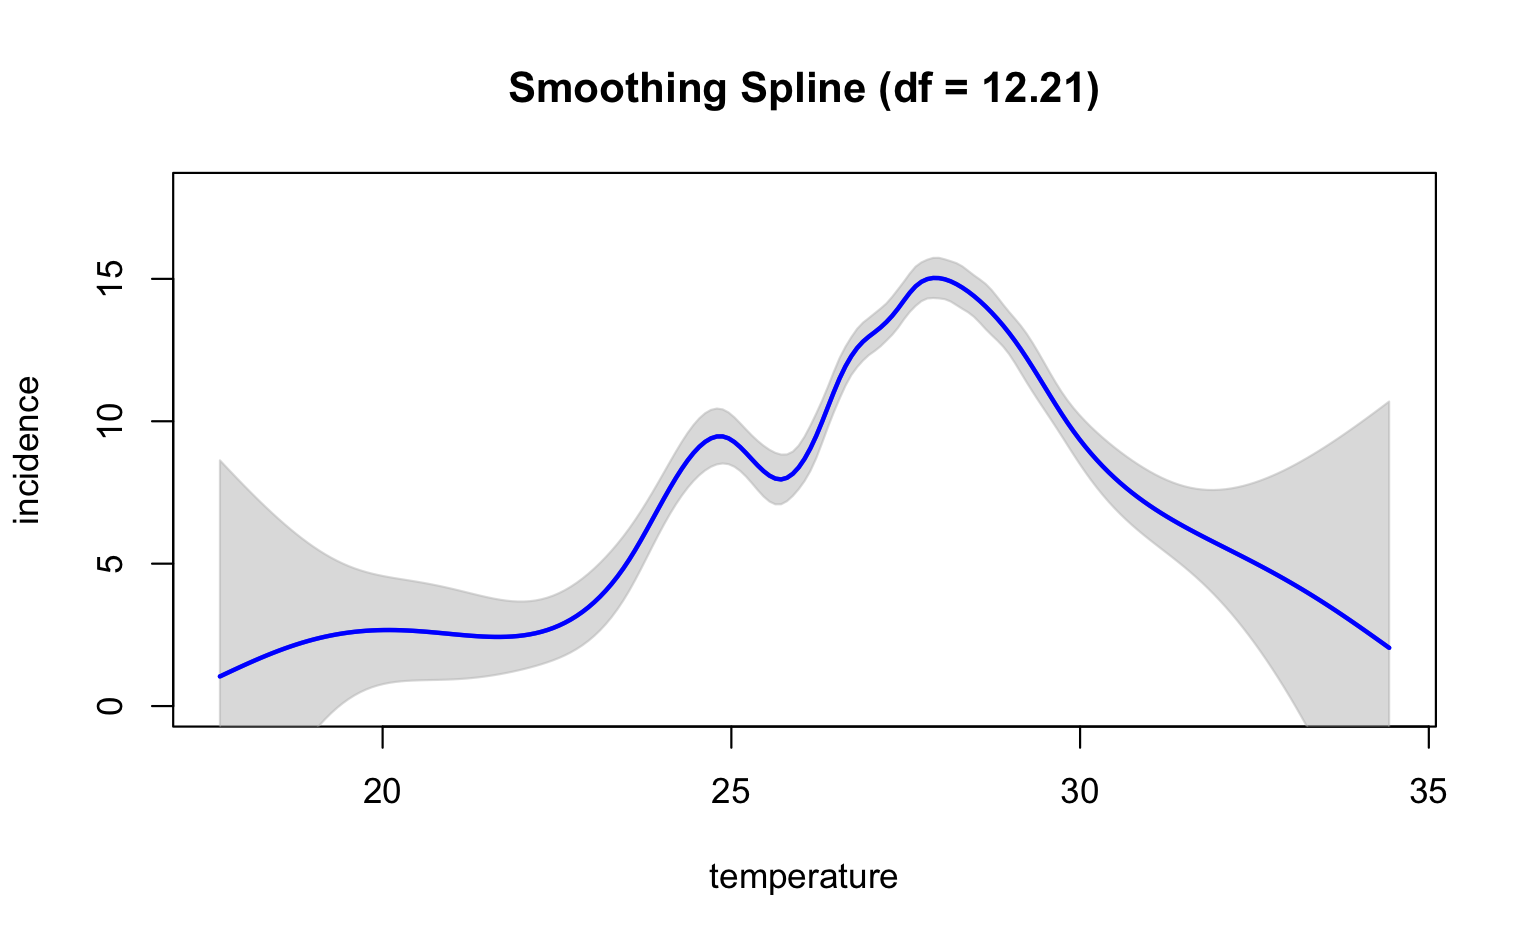
\includegraphics[width=0.7\textwidth]{fig/Smoothing_spline.png}
	\caption{Smoothing spline of incidences over temperature}
	\label{fig:smooth_spline}
\end{figure}

Computing the Pearson correlation between average dengue cases per year of whole Thailand and average temperature per year of whole Thailand a result of 0.43 is obtained. This suggests a moderate positive linear relationship. 

	\subsection{Time series decomposition}The time series of total dengue cases in Thailand was additively decomposed in the components trend, seasonal and random, as shown in Figure \ref{fig:decomp_ts_dengue}. The time series shows a seasonal pattern with a frequency of 12 months. The trend shows fluctuation over the time period with two periods of comparatively high dengue cases in 2013/14 and 2015/16.
	
	\begin{figure}[htbp] 
		\centering
		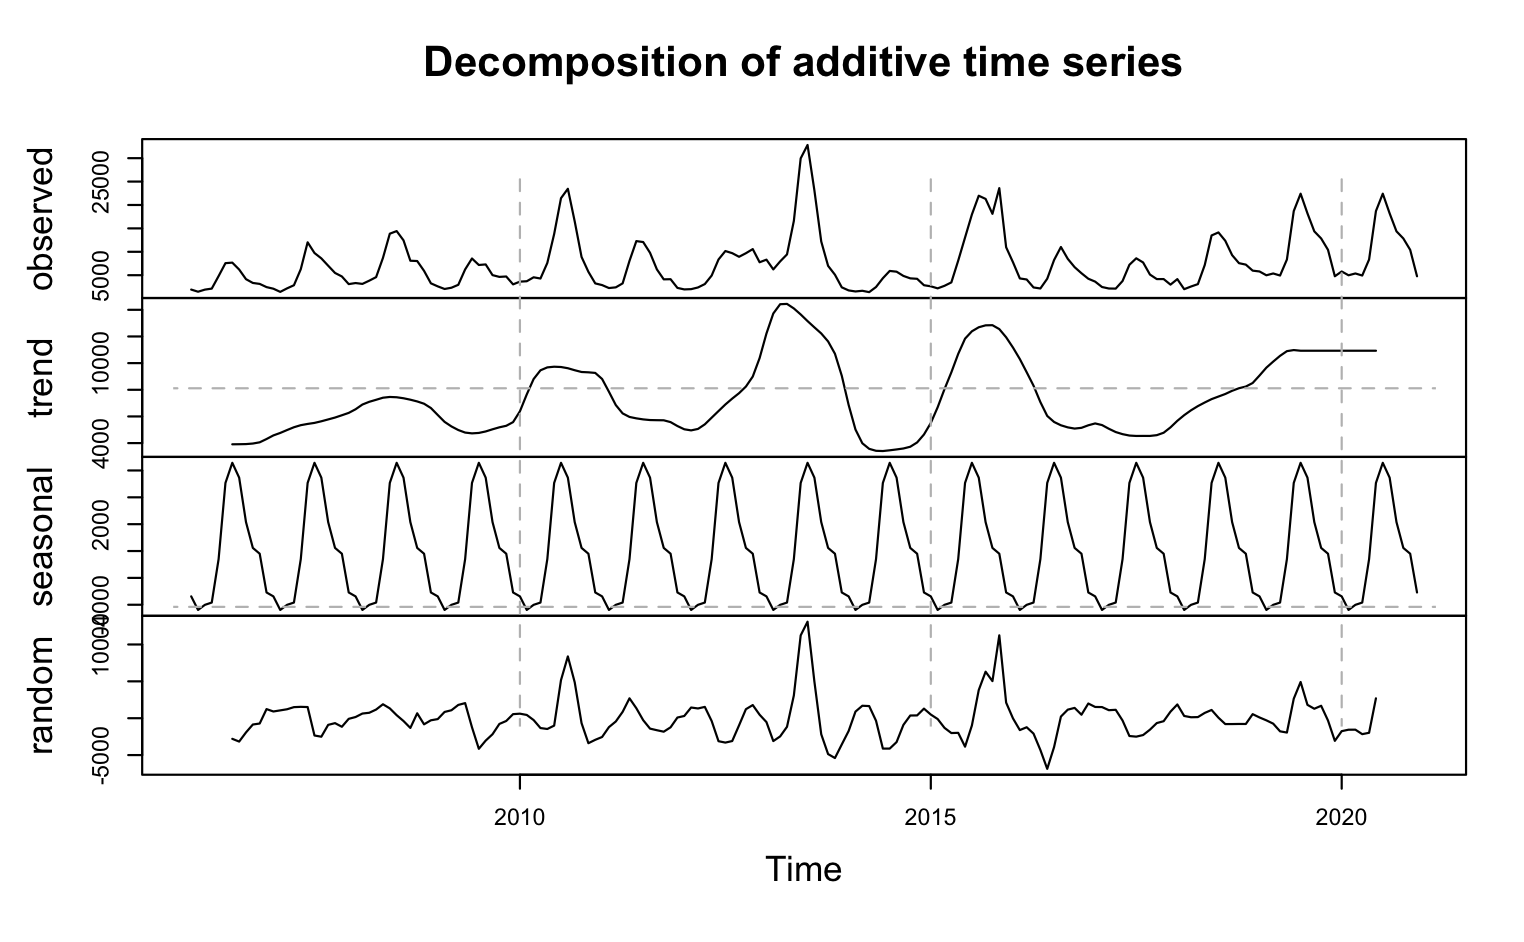
\includegraphics[width=0.7\textwidth]{fig/Decomposition_of_add_ts.png}
		\caption{ Decomposition of the additive time series of the total dengue cases in Thailand}
		\label{fig:decomp_ts_dengue}
	\end{figure}
	
	The decomposition of the time series of the dengue cases was compared to the decomposition of the time series of temperatures. Both time series have an annual seasonal pattern. The trends show in general similar patterns with differences in the amplitudes and slight shifts on the time axis, as shown in Figure \ref{fig:Trend_temp_cases}.
	\begin{figure}[hbpt] 
		\centering
		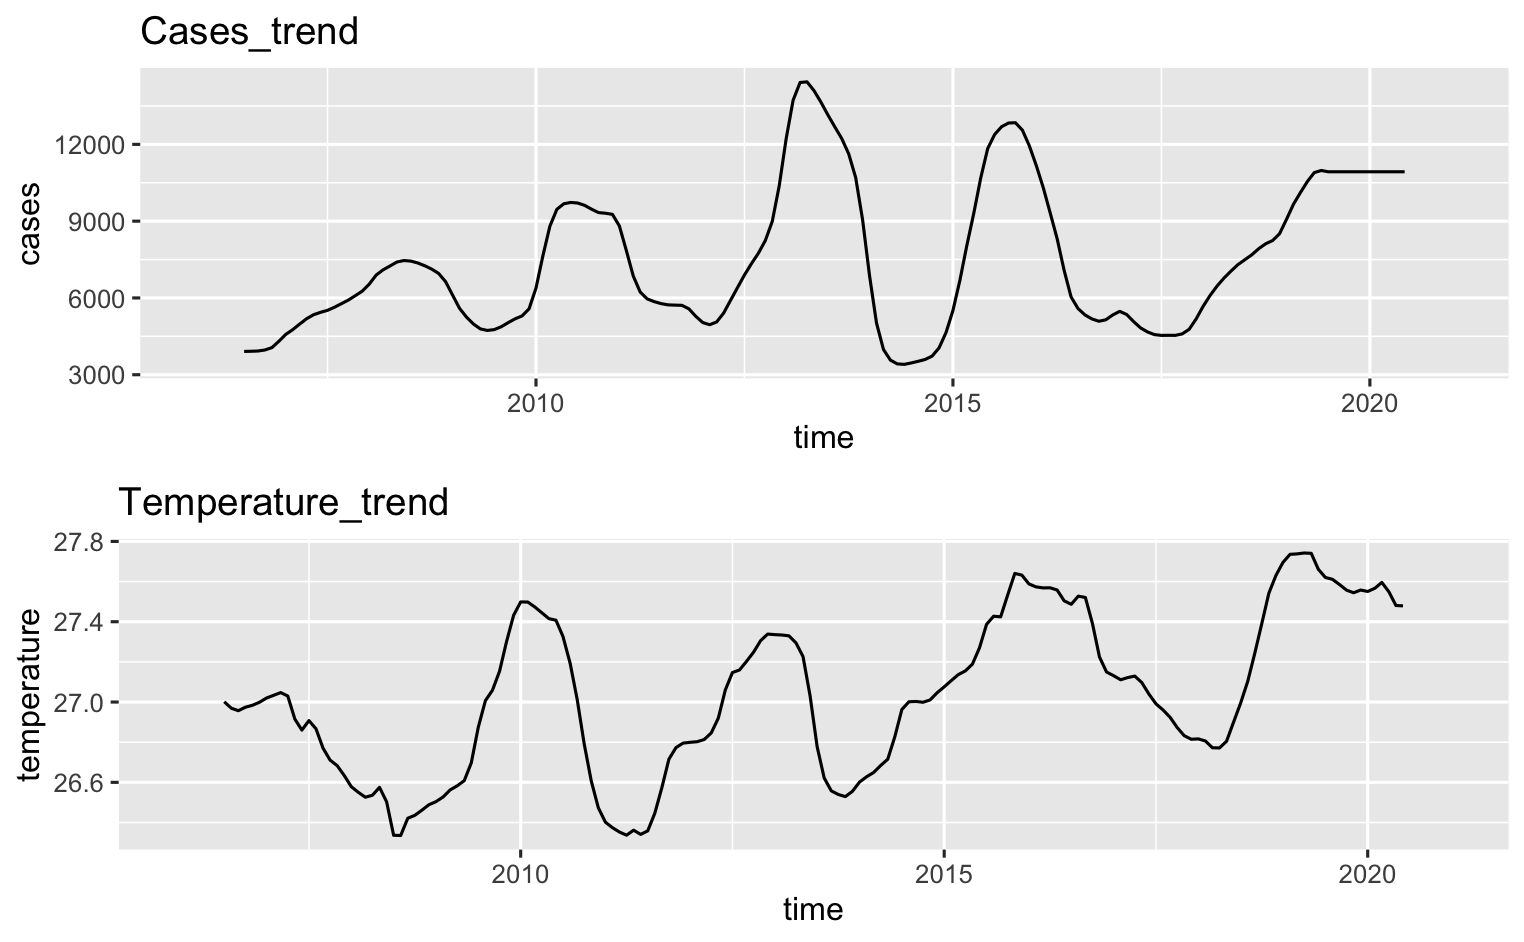
\includegraphics[width=0.7\textwidth]{fig/Trend_temp_cases.png}
		\caption{Trend of the total dengue cases in Thailand compared to the trend of the average temperature in Thailand for the years 2006 till 2020.}
		\label{fig:Trend_temp_cases}
	\end{figure}
	 In 2010 and 2012/13, there were temperature peaks, followed by peaking dengue cases a few months after. In 2015/16 rising temperatures were accompanied by rising dengue cases. 

	\subsection{ARIMA model and forecast}
	
	ARIMA modeling was performed to forecast the dengue case development in Thailand. For ADF test results, a p-value of 0.01 was used, for the KPSS test results a p-value of 0.1 was used. Therefore both test indicate stationarity of the time series and differencing isn’t necessary. Observation of the time series ACF showed oscillations which suggests the presence of seasonality in the data. The pACF exhibits a notable pattern with an initial positive peak followed by a significant negative peak. This pattern indicates the need to consider both autoregressive and moving average components in the model.
	To test for the optimal ARIMA model, models with different combinations of p, d and q values were generated and the best model was selected by comparing the AICs. The best model was found to be (2,2,2) with an AIC of 3319.732. Because this method could not account for seasonality in the data, the auto.arima function was used. “ARIMA(1,0,2)(1,1,0)[12] with drift” was found to be the best model. This model consists of an autoregressive term and two moving average terms. No differencing was performed. The model also has seasonal compounds with a period of 12. “With drift” means that a constant is included in the model. As the AIC of 3108.35 is lower and thus more accurate than the AIC of the former model, the auto.arima model was used for further analysis. 
	The evaluation of the histogram of the residuals revealed that the residuals were distributed similar to a normal distribution. The ACF plot indicates some significant autocorrelation at lag 1, while the remaining lags show no significant autocorrelation. The p-value of the Ljung-Box test was 0.41. Thus, the residuals are not distinguishable from white noise and the model has adequately captured the information in the data. 
	Based on the model, a forecast was made for the next four years, which extends beyond the data (see Figure \ref{fig:Auto_ARIMA_forecast}). 
	
		\begin{figure}[hbpt] 
		\centering
		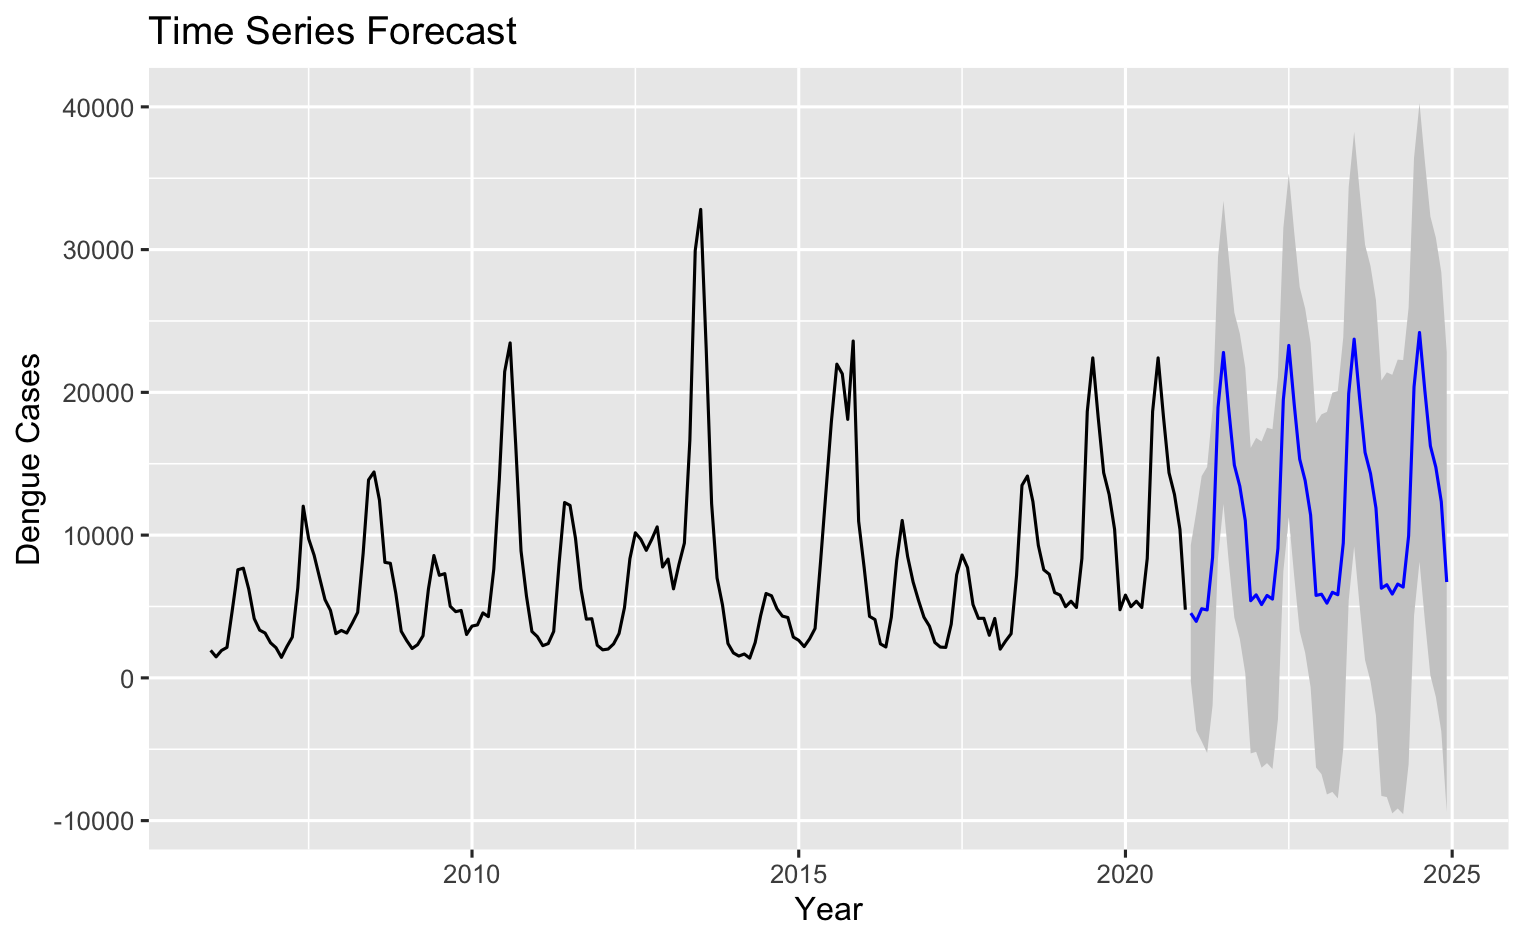
\includegraphics[width=0.7\textwidth]{fig/Auto_ARIMA_forecast.png}
		\caption{ARIMA forecast of the dengue cases in Thailand for 2021-2024.}
		\label{fig:Auto_ARIMA_forecast}
	\end{figure}
 
	To compare the accuracy of the forecast, the time series was cropped after December 2016 and the years 2017 till 2020 were forecasted, as shown in Figure \ref{fig:Auto_ARIMA_2016}. 
		\begin{figure}[hbpt] 
		\centering
		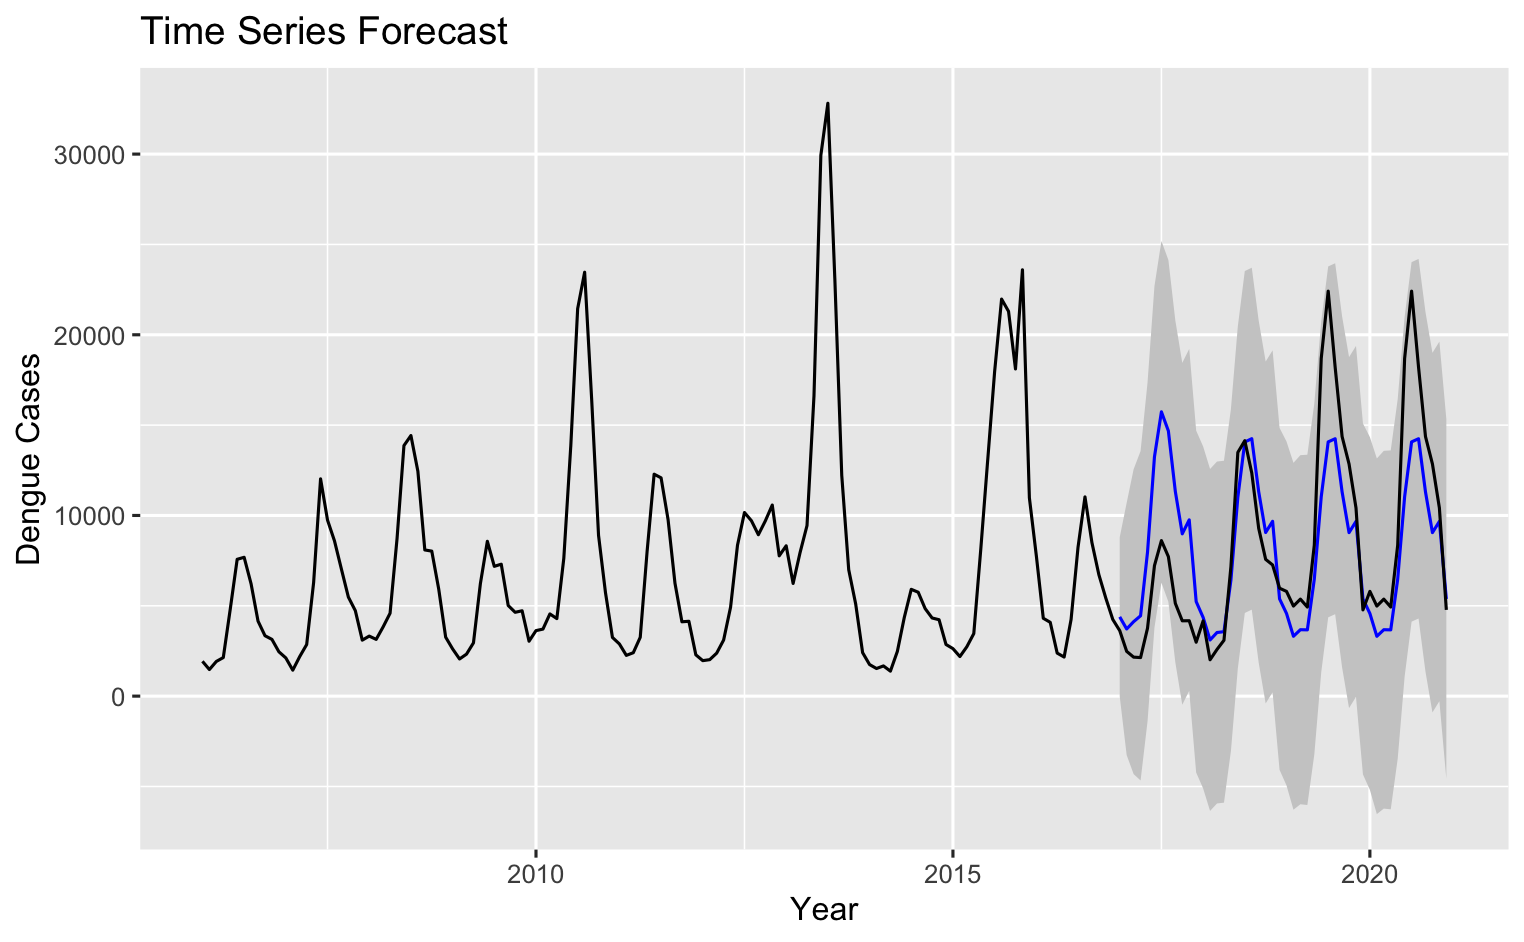
\includegraphics[width=0.7\textwidth]{fig/Auto_ARIMA_2016.png}
		\caption{ARIMA forecast of the dengue cases in Thailand for the years 2017-2020 (blue) compared to the actual dengue cases (black).}
		\label{fig:Auto_ARIMA_2016}
	\end{figure}

Although the forecast is more uniform than the actual cases in th years 2017 to 2020, the reported cases are in the range of deviation shown in grey. 

\subsection{GAM model}
A GAM model was generated based on the monthly temperature and incidence of all provinces of Thailand over the years 2006 - 2020. The predictor value (temperature) was passed into a smoothing function to create a smoothed spline curve. For the response variable (incidence) a quasi-Poisson distribution was chosen. The link function is a log transformation.

To figure out the optimal model, the degrees of freedom of the smoothing function were alternated. The effective degrees of freedom, which were found to be 13.82, resemble the complexity of the smooth curve. This value is relatively high, which indicates a “wigglier” spline. F-value and p-value indicate the statistical significance of the smooth function. In this case, the smooth function of temperature is highly significant (p-value $<$ 2e-16). The computed R-squared value of 0.0465 indicates how well the model explains the variance in the dependent variable. Here, the model explains approximately 4,7\% of the variance in the data. A low GCV (Generalized Cross Validation) value suggests a good fit of the model. The generated model has a GCV of 11.77. Additionally, the AIC value of the smooth model (112947.1) was compared with that of a linear model (113361.2). The smooth model had a lower value, which indicates a better fit.

Taking all these parameters into account, the GAM was computed with a k of 16. The model and its relationship of temperature and incidence is shown in the appendix Figure ..., as well as the evaluating graphs.

Subsequently the model was used to predict the average dengue case incidences over the period of 2021 - 2040, based on forecasted average temperature. You can see the average incidences of the past and future in Figure \ref{fig:}.


\section{Discussion}
Our results show ... 


	

\bibliography{bib/essay.bib}

\end{document}

